\documentclass[12pt,a4paper,oneside]{article}
\usepackage{graphicx,amssymb,setspace,float,fancyhdr,listings,xcolor,placeins,xeCJK,tocloft,amsmath}
\setCJKmainfont[AutoFakeBold=3]{STFangsong} % CJK Font Setup
\usepackage[dvipsnames]{xcolor}
\renewcommand{\cftsecleader}{\cftdotfill{\cftdotsep}} % Enable dot leaders
\renewcommand{\cftdotsep}{1} % Adjust dot spacing (1 is for close dots; increase for more spacing)
\setcounter{tocdepth}{3} % Set table of contents depth
\setstretch{1.25}


% 设置页眉和页脚
\setlength{\headheight}{13.6pt} % 设置页眉高度
\addtolength{\topmargin}{-1.6pt} % 调整上边距
\pagestyle{fancy}
\fancyhf{}
\fancyhead[C]{\small Python} % 中间页眉
\fancyfoot[C]{\small \thepage} % 中间页脚
\author{}
% 设置代码高亮样式
\lstset{
    language=Python,                 % 代码语言
    title=\lstname,                  % 标题显示代码文件名
    captionpos=b,                    % 标题位置(b表示底部)
    % 基本样式
    basicstyle=\ttfamily\small,      % 代码字体样式和大小
    keywordstyle=\bfseries\color{NavyBlue}, % 关键字样式
    commentstyle=\itshape\color{red!50!green!50!blue!50}, % 注释样式
    stringstyle=\bfseries\color{PineGreen!90!black}, % 字符串样式
    emph={self},                     % 指定强调词
    emphstyle=\bfseries\color{Rhodamine}, % 强调词样式
    % 背景与框架设置
    backgroundcolor=\color{black!3}, % 背景色
    frame=shadowbox,                 % 框架样式(阴影框)
    frameround=fttt,                 % 圆角样式
    rulesepcolor=\color{red!20!green!20!blue!20}, % 阴影框的颜色
    rulecolor=\color{black},         % 框架线颜色
    % 行号设置
    numbers=left,                    % 行号位置
    numberstyle=\tiny,               % 行号字体样式
    stepnumber=1,                    % 行号间隔
    numbersep=5pt,                   % 行号与代码间距
    % 布局设置
    showspaces=false,                % 是否显示空格
    showstringspaces=false,          % 是否显示字符串中的空格
    showtabs=false,                  % 是否显示制表符
    tabsize=4,                       % 制表符宽度
    breaklines=true,                 % 自动换行
    breakatwhitespace=false,         % 仅在空格处换行(false则不限定)
    columns=flexible,                % 列样式
    % 代码块的边距与间距设置
    xleftmargin=1em,                 % 左边距
    xrightmargin=-2em,               % 右边距
    aboveskip=1em,                   % 代码块上方的间距
    framexleftmargin=2em,            % 阴影框左边距
    % 其他设置
    escapeinside=``,                 % 允许在代码块中使用 LaTeX 命令
    morekeywords={}                  % 自定义更多关键字
}

\title{
    \vspace*{-2cm} % 调整垂直间距,使图像顶格显示
    
\includegraphics[width=0.8\textwidth]{SYSULogo.pdf} \\[1em]
    \vfill % 添加弹性空间,使内容居中
    \LARGE \textbf{MATLAB第一次大作业} \\[1em]
    \Large
    \begin{tabular}{rl}
        \textbf{姓名:} & \textbf{陈海弘} \\
        \textbf{学号:} & \textbf{23354049}
    \end{tabular}
    \vfill % 添加弹性空间,使内容居中
}
\date{\Large 2024.12.1}

\begin{document}

\maketitle

\newpage
\tableofcontents
\newpage
\section{实验目的}
\begin{itemize}
    \item 学习最速下降法的基本原理和实现方法。
    \item 通过编程实现最速下降法,并观察其在不同参数下的收敛情况。
\end{itemize}
\section{最速下降法原理}


最速下降法是一种常见的无约束优化方法,其问题定义为:
\[
\min f(\mathbf{x}), \quad \mathbf{x} \in \mathbb{R}^n,
\]
其中目标函数 \(f\) 在 \(\mathbb{R}^n\) 上连续可微。

算法步骤如下:
\begin{enumerate}
    \item 给定起始点 \(\mathbf{x}_0\),设定一个阈值 \(\epsilon > 0\)(如 0.01)作为终止条件,循环标号 \(k = 0\);
    \item 计算搜索方向:
    \[
    \mathbf{p}_k = -\nabla f(\mathbf{x}_k),
    \]
    即沿负梯度方向搜索;
    \item 检查梯度大小:
    \[
    \|\mathbf{p}_k\| \leq \epsilon,
    \]
    若满足条件,则停止迭代,令 \(\mathbf{x}^* \approx \mathbf{x}_k\);
    \item 更新迭代点:
    \[
    \mathbf{x}_{k+1} = \mathbf{x}_k + \alpha_k \mathbf{p}_k,
    \]
    其中步长 \(\alpha_k\) 的定义为:
    \[
    \alpha_k = \frac{-\nabla f(\mathbf{x}_k)^T \mathbf{p}_k}{\mathbf{p}_k^T \nabla^2 f(\mathbf{x}_k) \mathbf{p}_k}.
    \]
    \item 设置 \(k = k + 1\),返回步骤 2。
\end{enumerate}

\section{最速下降法实现}
我们使用 MATLAB 实现最速下降法,以下为代码思路分解:

\subsection*{1. 定义目标函数及其梯度}
目标函数 \(f(\mathbf{x})\) 和梯度函数 \(\nabla f(\mathbf{x})\) 定义为:
\[
f(\mathbf{x}) = 2x_1^2 + 4x_2^2 - 6x_1 - 2x_1x_2,
\]
\[
\nabla f(\mathbf{x}) = 
\begin{bmatrix}
4x_1 - 6 - 2x_2 \\
8x_2 - 2x_1
\end{bmatrix}.
\]
目标是找到使 \(f(\mathbf{x})\) 最小化的点 \(\mathbf{x}^*\)。


\subsection*{2. 初始化参数}
\begin{itemize}
    \item 初始点:\(\mathbf{x}_0 = \begin{bmatrix}0 \\ 0\end{bmatrix}\),作为迭代的起始点;
    \item 收敛容忍度:\(\text{tol} = 10^{-6}\),当 \(\|\nabla f(\mathbf{x}_k)\| < \text{tol}\) 时,算法认为已收敛;
    \item 最大迭代次数:\(\text{max\_iter} = 100\),限制迭代次数以防止死循环;
    \item 步长:\(\alpha = 0.1\),一个固定的更新步长,用于控制移动的幅度。
\end{itemize}


\subsection*{3. 迭代过程}
在每次迭代中执行以下步骤:
\begin{enumerate}
    \item \textbf{计算梯度:}  
    计算当前点 \(\mathbf{x}_k\) 的梯度:
    \[
    \mathbf{g}_k = \nabla f(\mathbf{x}_k).
    \]
    例如,若 \(\mathbf{x}_k = \begin{bmatrix}1 \\ 2\end{bmatrix}\),则:
    \[
    \mathbf{g}_k = 
    \begin{bmatrix}
    4(1) - 6 - 2(2) \\
    8(2) - 2(1)
    \end{bmatrix}
    =
    \begin{bmatrix}
    -6 \\
    14
    \end{bmatrix}.
    \]

    \item \textbf{检查收敛条件:}  
    若 \(\|\mathbf{g}_k\| < \text{tol}\),则认为当前点 \(\mathbf{x}_k\) 已接近最优解,停止迭代。梯度的范数定义为:
    \[
    \|\mathbf{g}_k\| = \sqrt{\sum_{i=1}^n g_{k,i}^2}.
    \]
    例如,当 \(\mathbf{g}_k = \begin{bmatrix}-6 \\ 14\end{bmatrix}\) 时:
    \[
    \|\mathbf{g}_k\| = \sqrt{(-6)^2 + 14^2} = \sqrt{36 + 196} = \sqrt{232}.
    \]

    \item \textbf{确定搜索方向:}  
    搜索方向为负梯度方向:
    \[
    \mathbf{d}_k = -\mathbf{g}_k.
    \]
    例如,当 \(\mathbf{g}_k = \begin{bmatrix}-6 \\ 14\end{bmatrix}\) 时:
    \[
    \mathbf{d}_k = 
    \begin{bmatrix}
    6 \\
    -14
    \end{bmatrix}.
    \]

    \item \textbf{更新迭代点:}  
    根据步长 \(\alpha\) 更新 \(\mathbf{x}_k\):
    \[
    \mathbf{x}_{k+1} = \mathbf{x}_k + \alpha \mathbf{d}_k.
    \]
    例如,若 \(\mathbf{x}_k = \begin{bmatrix}1 \\ 2\end{bmatrix}\),\(\alpha = 0.1\),\(\mathbf{d}_k = \begin{bmatrix}6 \\ -14\end{bmatrix}\),则:
    \[
    \mathbf{x}_{k+1} = \begin{bmatrix}1 \\ 2\end{bmatrix} + 0.1 \begin{bmatrix}6 \\ -14\end{bmatrix} = \begin{bmatrix}1.6 \\ 0.6\end{bmatrix}.
    \]

    \item \textbf{增加迭代计数器:}  
    令 \(k = k + 1\),并返回步骤 (1)。
\end{enumerate}


目标函数为:
\[
f(x_1, x_2) = 2x_1^2 + 4x_2^2 - 6x_1 - 2x_1x_2
\]

梯度公式为:
\[
\nabla f(x_1, x_2) = 
\begin{bmatrix}
4x_1 - 6 - 2x_2 \\
8x_2 - 2x_1
\end{bmatrix}
\]

初始点设为 $x_0 = (0, 0)$,步长 $\alpha = 0.1$,收敛条件为梯度模长小于 $10^{-6}$。

\subsection*{第一次迭代}

1. 当前点:
\[
x_0 = \begin{bmatrix} 0 \\ 0 \end{bmatrix}
\]

2. 计算梯度:
\[
\nabla f(x_0) = 
\begin{bmatrix}
4(0) - 6 - 2(0) \\
8(0) - 2(0)
\end{bmatrix} = 
\begin{bmatrix}
-6 \\
0
\end{bmatrix}
\]

3. 确定方向(负梯度方向):
\[
d_0 = -\nabla f(x_0) = 
\begin{bmatrix}
6 \\
0
\end{bmatrix}
\]

4. 更新点:
\[
x_1 = x_0 + \alpha \cdot d_0 = 
\begin{bmatrix}
0 \\
0
\end{bmatrix} + 0.1 \cdot 
\begin{bmatrix}
6 \\
0
\end{bmatrix} = 
\begin{bmatrix}
0.6 \\
0
\end{bmatrix}
\]

5. 更新目标函数值:
\[
f(x_1) = 2(0.6)^2 + 4(0)^2 - 6(0.6) - 2(0.6)(0) = -1.08
\]

\subsection*{第二次迭代}

1. 当前点:
\[
x_1 = \begin{bmatrix} 0.6 \\ 0 \end{bmatrix}
\]

2. 计算梯度:
\[
\nabla f(x_1) = 
\begin{bmatrix}
4(0.6) - 6 - 2(0) \\
8(0) - 2(0.6)
\end{bmatrix} = 
\begin{bmatrix}
-3.6 \\
-1.2
\end{bmatrix}
\]

3. 确定方向(负梯度方向):
\[
d_1 = -\nabla f(x_1) = 
\begin{bmatrix}
3.6 \\
1.2
\end{bmatrix}
\]

4. 更新点:
\[
x_2 = x_1 + \alpha \cdot d_1 = 
\begin{bmatrix}
0.6 \\
0
\end{bmatrix} + 0.1 \cdot 
\begin{bmatrix}
3.6 \\
1.2
\end{bmatrix} = 
\begin{bmatrix}
0.96 \\
0.12
\end{bmatrix}
\]

5. 更新目标函数值:
\[
f(x_2) = 2(0.96)^2 + 4(0.12)^2 - 6(0.96) - 2(0.96)(0.12) = -1.872
\]

\subsection*{一般步骤}
重复上述过程,直到梯度模长 $\|\nabla f(x)\| < 10^{-6}$,最终得到最优点和最小值。

\subsection*{4. 收敛与输出}
当满足收敛条件或达到最大迭代次数时,返回结果:
\begin{itemize}
    \item 最优点:
    \[
    \mathbf{x}^* = \mathbf{x}_k.
    \]
    \item 最优值:
    \[
    f^* = f(\mathbf{x}_k).
    \]
    \item 迭代次数:
    \[
    \text{iter} = k.
    \]
\end{itemize}
例如,若最终 \(\mathbf{x}_k = \begin{bmatrix}1.5 \\ 1.5\end{bmatrix}\),则:
\[
f^* = f(1.5, 1.5) = 2(1.5)^2 + 4(1.5)^2 - 6(1.5) - 2(1.5)(1.5) = -2.25.
\]
代码实现:
\begin{lstlisting}
    function steepest_descent_custom
    f = @(x) 2*x(1)^2 + 4*x(2)^2 - 6*x(1) - 2*x(1)*x(2); 
    grad_f = @(x) [4*x(1) - 6 - 2*x(2); 8*x(2) - 2*x(1)];
    x0 = [0; 0];       
    tol = 1e-6;        
    max_iter = 100;   
    alpha = 0.1;       
    [x_min, f_min, iter] = steepest_descent_solver(f, grad_f, x0, tol, max_iter, alpha);
    fprintf('最优点: (%.6f, %.6f)\n', x_min(1), x_min(2));
    fprintf('最优值: %.6f\n', f_min);
    fprintf('迭代次数: %d\n', iter);
end

function [x, fval, iter] = steepest_descent_solver(f, grad_f, x0, tol, max_iter, alpha)
    x = x0;
    iter = 0;
    while iter < max_iter
        grad = grad_f(x);
        if norm(grad) < tol
            break; 
        end

        d = -grad; 
        x = x + alpha * d; 
        iter = iter + 1;
    end

    fval = f(x); 
end
\end{lstlisting}

结果:
\begin{figure}[H]
    \centering
    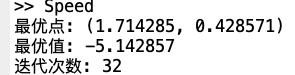
\includegraphics[width=0.5\textwidth]{image/1.png}
    \caption{最速下降法结果}
\end{figure}
可以看到,最速下降后收敛到1.7,0.42这个点,迭代次数32。
\section{总结}
这次作业学习了最速下降法在matlab中的实现,首先定义了目标函数和梯度函数,然后初始化参数,接着进行迭代,最后输出结果。a

最速下降法的原理就是沿负梯度方向搜索,直到满足收敛条件,详细来说就是给定一个初始点,然后计算该点的梯度,确定搜索方向,然后更新迭代点,直到满足收敛条件。

对我来说,难点在于matlab代码的编写,虽然之前有接触过matlab,但是对其语法并不熟悉,所以编写代码花费了较多的时间。比如:
\begin{itemize}
    \item 函数定义时,需要使用@符号来定义匿名函数。
    \item 在迭代过程中,需要使用while循环来实现迭代,并且需要使用break语句来跳出循环。
    \item 在更新迭代点时,需要使用x = x + alpha * d来更新迭代点。
\end{itemize}
\end{document}